\subsection{Dallamszerkesztés az akkord vertikális értelmezésével}
\label{sec:exdallamvert}
Szerkesszünk dallamot A-dúr hangnemben, a hangnem akkordjainak kíséretére!
\begin{pitemize}
Funkció & T & ST(SD) & M(D,T) & SD & D & SM(SD,T) & V(D) \\ \hline
Az skála hangjai & \key{A} & \key{H} & \key{Cs} & \key{D} & \key{E} & \key{Fs} & \key{Gs} \\
Hármashangzatai & \chord{A} & \chord{Hm} & \chord{Csm} & \chord{D} & \chord{E} & \chord{Fsm} & \chord{GsO} \\
Négyeshangzatai & \chord{Amaj7} & \chord{Hm7} & \chord{Csm7} & \chord{Dmaj7} & \chord{E7} & \chord{Fsm7} & \chord{Gso7} \\
\end{pitemize}
Horizontális felfogásban a skála akkordjait a skála hangjaiból álló dallam kíséri.
Hogy egy kicsit érdekesebben hangozzék, két ütemen keresztül a funkciót vertikálisan értelmezzük.
A következő lépés azon skálák meghatározása, melyekben az általunk kiválasztott kísérő akkordok szerepelnek. Ezúttal legyen ez a domináns \chord{E7}.
Vizsgáljuk meg a fokokról induló akkordok típusait a ,,\nameref{sec:skalaakkordok}'' mellékletben. \\\\
A melodikus moll skála negyedik fokán, a kulcshangtól kvart távolságra elhelyezkedő 
\chord{E7}-hez a hangközfordítás szabályai szerint a kulcshang \key{E}-től tiszta kvint távolságra van,
tehát a keresett skála a \scale{H}{m}: 
\key{H}, \key{Cs}, \key{D}, \key{E}, \key{Fs}, \key{Gs}, \key{As}. \\\\
A melodikus moll skála ötödik fokán, a kulcshangtól kvint távolságra elhelyezkedő 
\chord{E7}-hez a hangközfordítás szabályai szerint a kulcshang \key{E}-től tiszta kvart távolságra van,
tehát a keresett skála az \scale{A}{m}:
\key{A}, \key{H}, \key{C}, \key{D}, \key{E}, \key{Fs}, \key{Gs}. \\\\
A harmonikus moll skála ötödik fokán, a kulcshangtól kvint távolságra elhelyezkedő 
\chord{E7}-hez a hangközfordítás szabályai szerint a kulcshang \key{E}-től tiszta kvart távolságra van,
tehát a keresett skála az \scale{A}{m}:
\key{A}, \key{H}, \key{C}, \key{D}, \key{E}, \key{F}, \key{Gs}. \\\\
Az utolsó kettőből és az alapskálából alkotott kilenc fokú alterált skála:
\key{A}, \key{H}, \key{C}, \key{Cs}, \key{D}, \key{E}, \key{F}, \key{Fs}, \key{Gs} \\\\
Pillér hangok \chord{E7}-hez:
\key{E}, \key{Gs}, \key{H}, \key{D} \\
Diatonikus váltóhangok (a kísérő akkord hangjait elhagyva):
\key{A}, \key{C}, \key{Cs}, \key{F}, \key{Fs} \\
Kromatikus váltóhangok:
(\key{E}-hez) \key{Ds},
(\key{Gs}-hez) \key{G}, \key{As},
(\key{H}-hoz) \key{As},
(\key{D}-hez) \key{Ds}. \\\\
Az első öt ütem horizontális értelmezés szerint a skála hangjaival kísért akkordokat tartalmaz. A következő kettő érdekesebben hangzik: a dallammenet  \key{E} - \key{As} - \key{H} - \key{D}, \key{Gs} - \key{F} - \key{H} - \key{Gs}. Szerkezete PH - KV - PH - PH, PH - DV - PH - PH. . A dallam a ,,\nameref{fig:notevertical}'' kottán látható.

\subsection{Dallamszerkesztés enharmonikus kiegészítéssel}
\label{sec:exdallamenharm}
Az előbbi példában leírt akkord kíséretre most írjunk dallamot az \chord{E7} akkord enharmonikusaihoz tartozó skálákból! \\\\
\key{E}, \textcolor{red}{\key{Gs}, \key{H} és \key{D}} $\longrightarrow$ \chord{GsO} \\
\textcolor{red}{\key{H} és \key{D}} + \key{Fs} $\longrightarrow$ \chord{Hm} \\
\textcolor{red}{\key{H} és \key{D}} + \key{F} $\longrightarrow$ \chord{HO} \\
\key{Cs} + \textcolor{red}{\key{E} és \key{Gs}} $\longrightarrow$ \chord{Csm} (\key{Cs}-moll skála)\\
\key{C} + \textcolor{red}{\key{E} és \key{Gs}} $\longrightarrow$ \chord{C+} \\
\key{A}, \key{Cs} + \textcolor{red}{\key{E} és \key{Gs}} $\longrightarrow$ \chord{Amaj7} (\key{A} dúr skála) \\
\key{As}, \key{Cs} + \textcolor{red}{\key{E} és \key{Gs}} $\longrightarrow$ \chord{Aso} \\
\textcolor{red}{\key{Gs}, \key{H}}, \key{D} $\longrightarrow$ \chord{Gsm} \\
\key{A}, \key{C}, \textcolor{red}{\key{E}, \key{Gs}} $\longrightarrow$ \chord{Ammaj7} (\key{A} moll skála) \\\\
A fenti lehetőségek közül válasszuk a \scale{Cs}{m} és az \scale{A}{} skálákat - ezek uniója: \key{E}, \key{Fs}, \key{Gs}, \key{A}, \key{H}, \key{C}, \key{Cs}, \key{D}, \key{Ds}. Az ötödik, hatodik és hetedik ütemben ennek a skálának a hangjait használjuk, ügyelve arra, hogy az első és a harmadik ütem pillér hanggal kezdődjön. A dallam a ,,\nameref{fig:noteenharmonic}'' kottán látható.
 
\begin{figure}[!htbp]
 \advance\leftskip-6mm
 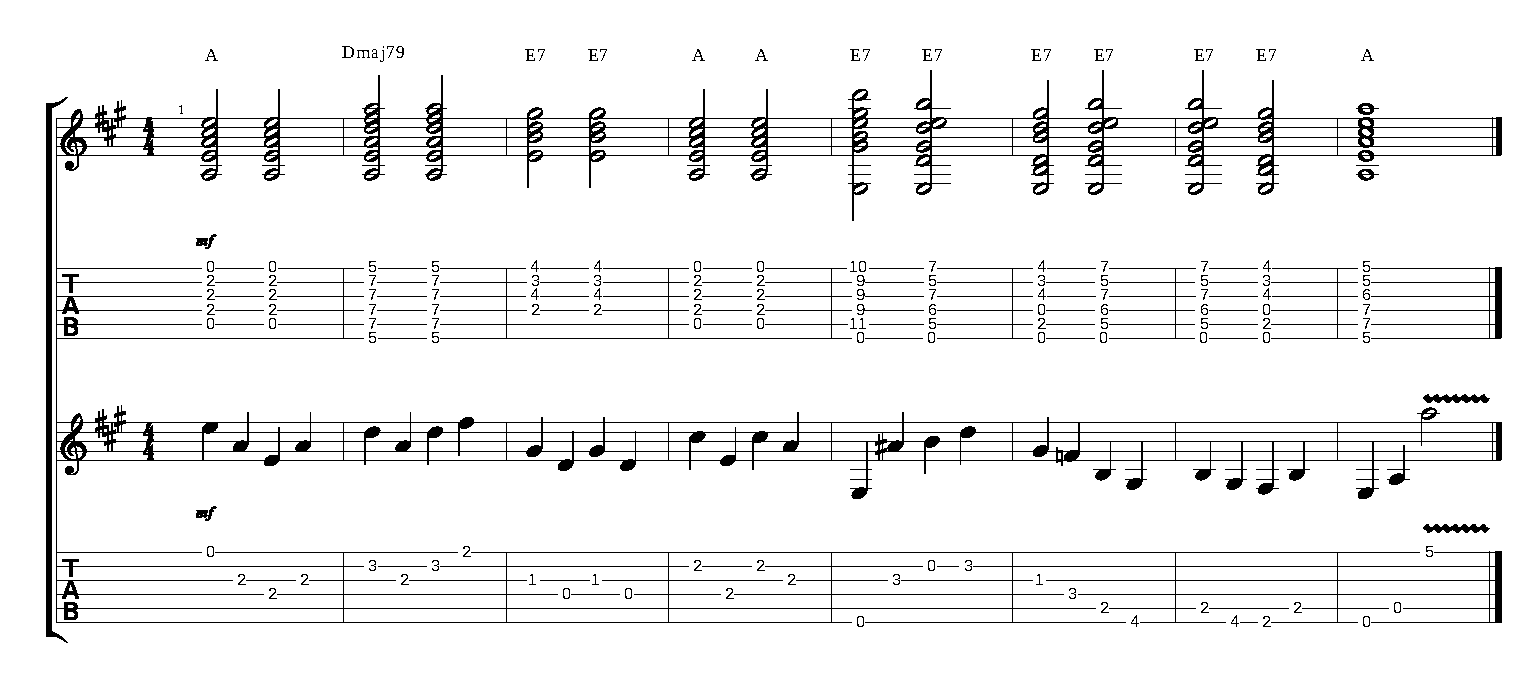
\includegraphics[page=1,scale=0.70]{notes/dallamszerkesztes.pdf}
 \captionof{figure}{Vertikális értelmezéssel színezett dallammenet}
 \label{fig:notevertical}
\end{figure}

\begin{figure}[!htbp]
 \advance\leftskip-6mm
 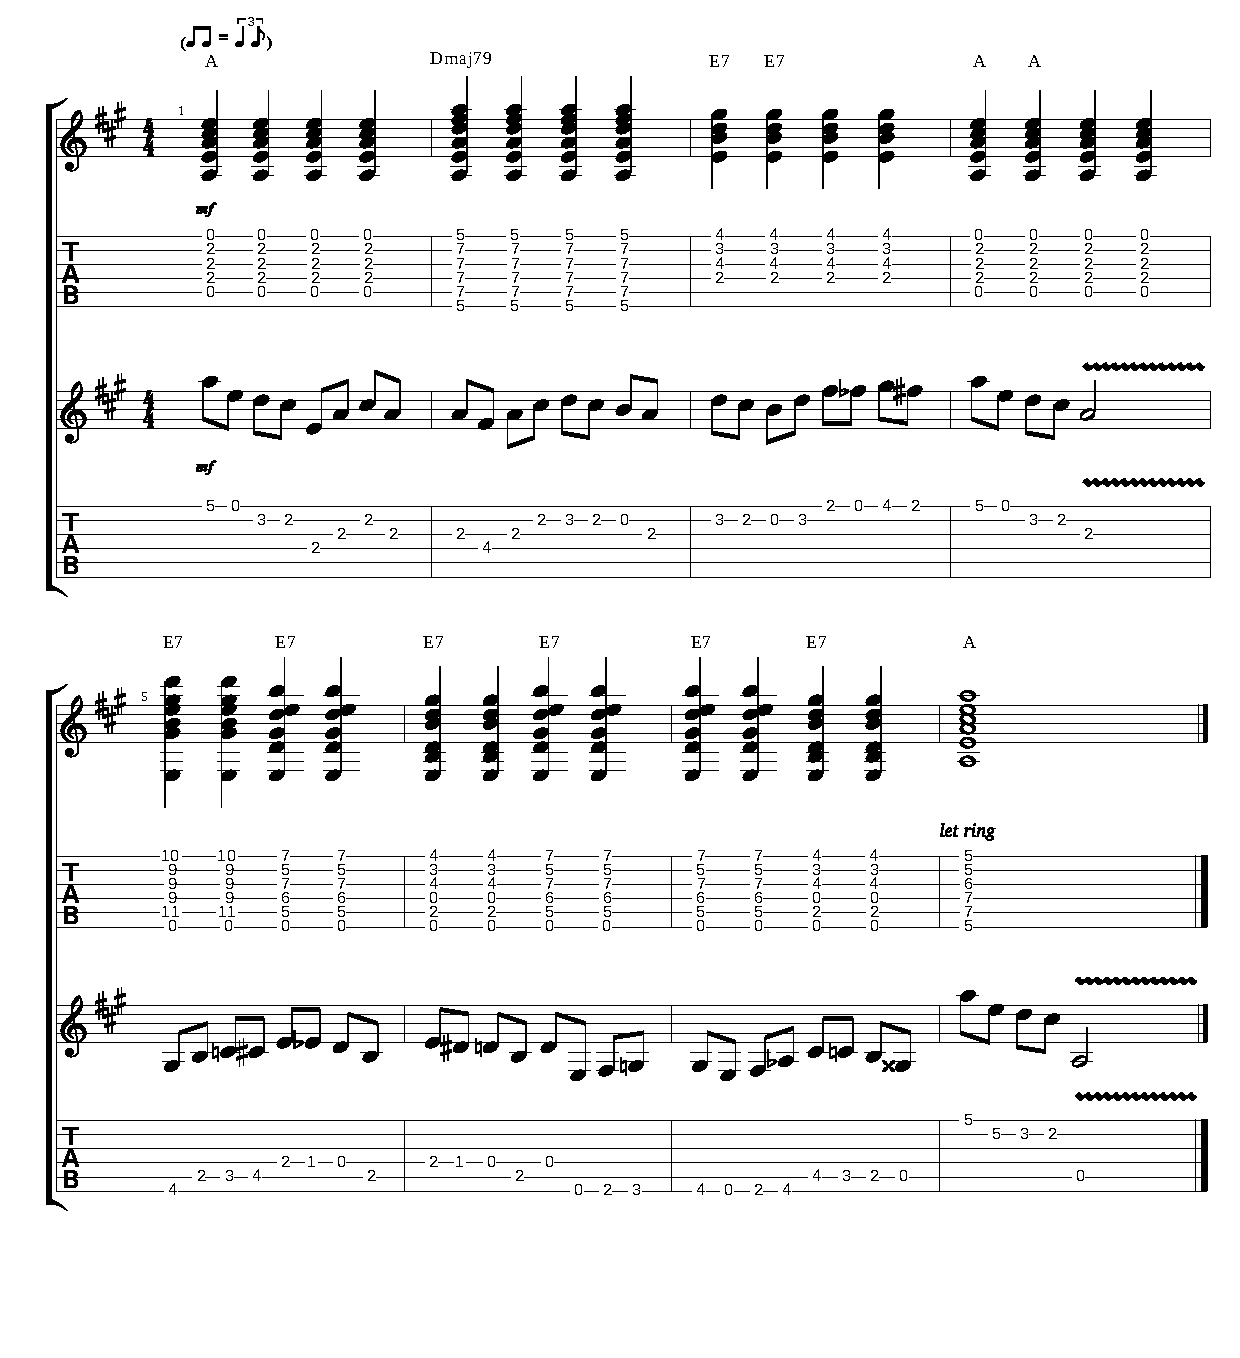
\includegraphics[page=1,scale=0.85]{notes/dallamszerkesztes_II.pdf}
 \captionof{figure}{Enharmonikus kiegészítéssel színezett dallammenet}
 \label{fig:noteenharmonic}
\end{figure}
